The final application demonstrating the power of \gpmem\ illustrates its use in Bayesian optimization. We introduce Thompson sampling, the basic solution strategy
underlying the Bayesian optimization with \gpmem.
Thompson sampling~\cite{thompson1933likelihood} is a widely used Bayesian
framework for addressing the trade-off between exploration and exploitation in
multi-armed (or continuum-armed) bandit problems.  
We cast the multi-armed bandit problem as a one-state Markov
decision process (MDP), and describe how Thompson sampling can be used to choose
actions for that MDP.

The MDP is as follows: An agent is to take a sequence of actions $a_1, a_2,
\ldots$ from a (possibly infinite) set of possible actions $\Acal$.  After each
action, a reward $r \in \R$ is received, according to an unknown conditional
distribution $P_\true\pn{r \mvert a}$.  The agent's goal is to maximize the
total reward received for all actions in an online manner.  In Thompson
sampling, the agent accomplishes this by placing a prior distribution
$P(\ttheta)$ on the possible ``contexts'' $\ttheta \in \Theta$.  Here a context
is a believed model of the conditional distributions $\{P\pn{r \mvert a}\}_{a
\in \Acal}$, or at least, a believed statistic of these conditional
distributions which is sufficient for deciding an action $a$.  If actions are
chosen so as to maximize expected reward, then one such sufficient statistic is
the believed conditional mean $V \pn{a \mvert \ttheta} = \Ebkt{r \mvert
a;\ttheta}$, which can be viewed as a believed value function.  For
consistency with what follows, we will assume our context $\ttheta$ takes the
form $(\thetabf, \abf, \rbf)$ where $\abf$ is the vector of past
actions, $\rbf$ is the vector of their rewards, and $\bm{\theta}$ (the
``semicontext'') contains any other information that is included in the context.

In this setup, Thompson sampling has the following steps:
\begin{algorithm}[H]
  \singlespacing
  Repeat as long as desired:
  \begin{enumerate}
    \item\label{itm:thompson-step-sample} {\bf Sample.} Sample a semicontext
      $\thetabf \sim P(\thetabf)$.
    \item\label{itm:thompson-step-search} {\bf Search (and act).} Choose an
      action $a \in \Acal$ which (approximately) maximizes $V\pn{a \mvert
      \ttheta} = \Ebkt{r \mvert a; \ttheta} = \Ebkt{r \mvert a;\,\thetabf,
      \abf, \rbf}$.
    \item {\bf Update.} Let $r_\true$ be the reward received for action $a$.
      Update the believed distribution on $\thetabf$, i.e., $P(\thetabf) \gets
      P_\rmnew(\thetabf)$ where $P_\rmnew(\thetabf) = P\pn{\thetabf \mvert a \mapsto
      r_\true}$.
  \end{enumerate}
  \caption{Thompson sampling.}
  \label{alg:thompson}
\end{algorithm}
Note that when $\Ebkt{r|a;\ttheta}$ (under the sampled value of $\thetabf$ for
some points $a$) is far from the true value $\Ebkt[P_\true]{r \mvert a}$, the
chosen action $a$ may be far from optimal, but the information gained by probing
action $a$ will improve the belief $\ttheta$.  This amounts to ``exploration.''
When $\Ebkt{r \mvert a;\ttheta}$ is close to the true value except at points $a$
for which $\Ebkt{r \mvert a;\ttheta}$ is low, exploration will be less likely to
occur, but the chosen actions $a$ will tend to receive high rewards.  This
amounts to ``exploitation.'' The trade-off between exploration and exploitation
is illustrated in Figure \ref{fig:slide2}.  Roughly speaking, exploration will
happen until the context $\ttheta$ is reasonably sure that the unexplored
actions are probably not optimal, at which time the Thompson sampler will
exploit by choosing actions in regions it knows to have high value.

\begin{figure}
  \centering
\begin{overpic}[width=1.05\textwidth]{figs/slide2.pdf}
\put(150,300){{\parbox{0.4\linewidth}{%
    \tiny
    \begin{align*}
	E\pn{a' \mvert a} &= -\frac1s \pn{\widetilde{\mu}(a') -
	\widetilde{\mu}(a)} \\
	\widetilde{\mu}(a) &= \frac{1}{N_\avg} \sum_{i=1}^{N_\avg}
	\widetilde{r}_{i,a}i\\ 
	\widetilde{r}_{i,a}=\hat{f} &\sim \Ncal(\hat\mubf, \hat\Kbf\mid
\sigma,\ell,\abf,\rbf)\\ 
	Q_\proposal\pn{a' \mvert a} &\sim \Ncal(a,\,\propstd^2)
    \end{align*}}}}
\put(118,326){$\tau_\search$:}
\put(62,50){{\parbox{0.4\linewidth}{%
    \tiny
    \begin{align*}
  P(\sigma,\ell \mid \abf,\rbf) &\propto \exp \big \{ {-\frac{1}{2}}\rbf^\top
\Kbf(\abf,\abf)^{-1}\rbf \big \}\\
  Q_\proposal\pn{\sigma',\ell \mvert \sigma,\ell} &= P(\sigma')\\
  Q_\proposal\pn{\sigma,\ell' \mvert \sigma,\ell} &= P(\ell')\\
  P_\accept\pn{\sigma',\ell' \mvert \sigma,\ell,\abf,\rbf}
  &=
   \frac{
    P\pn{\sigma}P\pn{\ell}
    }{
    P\pn{\sigma'}P\pn{\ell'}
    } 
   \exp\bigg \{ {-\frac12}\big(
    \rbf^T \Kbf\pn{\abf, \abf \mvert \sigma', \ell'}^{{-1}} \rbf - 
    \rbf^T \Kbf\pn{\abf, \abf \mvert \sigma, \ell}^{{-1}} \rbf
  \big)\bigg \}\\
   K(\abf,\abf)&=\text{SE}=\bigg[\sigma^2 \exp \big \{{-\frac{(a_1 -
a_2)^2}{2\ell}}\big \}\bigg]_{a_1,a_2 \in \abf}
    \end{align*}}}}
\put(65,107){$\tau_\update$:}
\put(252,65){\bigg \} \footnotesize MH}
\put(250,85){ \} \footnotesize True posterior }
%\put(105,107){\footnotesize True Posterior}
%\put(105,90){\footnotesize MH:}
\end{overpic}
  \caption{
    Two possible actions (in green) for an iteration of Thompson sampling.  The
    believed distribution on the value function $V$ is depicted in red.  In this
    example, the true reward function is deterministic, and is drawn in blue.
    The action on the right receives a high reward, while the action on the left
    receives a low reward but greatly improves the accuracy of the believed
    distribution on $V$.  The transition operators $\tau_\search$ and
    $\tau_\update$ are described in Section \ref{sec:math-spec}.
  }
  \label{fig:slide2}
\end{figure}

Typically, when Thompson sampling is implemented, the search over contexts
$\ttheta \in \Theta$ is limited by the choice of representation.  In
traditional programming environments, $\thetabf$ often consists of a few
numerical parameters for a family of distributions of a fixed functional
form.  With work, a mixture of a few functional forms is possible; but
without probabilistic programming machinery, implementing a rich context
space $\Theta$ would be an unworkably large technical burden.  In a
probabilstic programing language, however, the representation of
heterogeneously structured or infinite-dimensional context spaces is quite
natural.  Any computable model of the conditional distributions
$\br{P\pn{r \mvert a}}_{a \in \Acal}$ can be represented as a stochastic
procedure $(\lambda (a) \ldots)$.  Thus, for computational Thompson sampling,
the most general context space $\widehat\Theta$ is the space of program texts.
Any other context space $\Theta$ has a natural embedding as a subset of
$\widehat\Theta$.
\myparagraph{A Mathematical Specification}\label{sec:math-spec}
We now describe a particular case of Thompson sampling with the following properties:
\begin{itemize}
  \item The regression function has a Gaussian process prior.
  \item The actions $a_1,a_2,\ldots \in \Acal$ are chosen by a Metropolis-like search
    strategy with Gaussian drift proposals.
  \item The hyperparameters of the Gaussian process are inferred using
    Metropolis--Hastings sampling after each action.
\end{itemize}

In this version of Thompson sampling, the contexts $\ttheta$ are Gaussian
processes over the action space $\Acal = [-20, 20] \subseteq \R$.  That is,
\[ V \sim \mathcal{GP}\big(\mubf(a), \Kbf(a,a)\big), \]
where the mean $\mubf$ is a computable function $\Acal \to \R$ and the covariance
$\Kbf$ is a computable (symmetric, positive-semidefinite) function $\Acal \times
\Acal \to \R$.  This represents a Gaussian process $\br{R_a}_{a \in \Acal}$,
where $R_a$ represents the reward for action $a$. We write past actions as
$\abf$ and past rewards as $\rbf$. Computationally, we represent
a context as a data structure
\[ \ttheta = (\thetabf, \abf, \rbf) = (\bm{\mu}, \Kbf,\thetabf, \abf, \rbf), \]
where $\mubf$ is a procedure to be used as the prior mean function and
$\Kbf$ is a procedure to be used as the prior covariance function, parameterized by 
$\thetabf$.
As above set $\bm{\mu} \equiv 0$.

Note that the context space $\Theta$ is not a finite-dimensional parametric
family, since the vectors $\abf$ and $\rbf$ grow as more samples are
taken.  $\Theta$ is, however, representable as a computational
procedure together with parameters and past samples, as we do in the
representation $\ttheta = (\mubf, \Kbf, \thetabf, \abf, \rbf)$.

We combine the Update and Sample steps of Algorithm \ref{alg:thompson} by
running a Metropolis--Hastings (MH) sampler whose stationary distribution is the
posterior $P\pn{\thetabf \mvert \abf, \rbf}$.  The functional forms of
$\mubf$ and $\Kbf$ are fixed in our case, so inference is only done
over the parameters $\thetabf = \br{\sigma,\ell}$; hence we equivalently write
$P\pn{\sigma,\ell \mvert \abf, \rbf}$ for the stationary
distribution.  We make MH proposals to one variable at a time, using the prior
as proposal distribution:
\[
  Q_\proposal\pn{\sigma',\ell \mvert \sigma,\ell} = P(\sigma')
\]
and
\[
  Q_\proposal\pn{\sigma,\ell' \mvert \sigma,\ell} = P(\ell').
\]
The MH acceptance probability for such a proposal is
\[
  P_\accept\pn{\sigma',\ell' \mvert \sigma,\ell}
  =
  \min\br{1,\ \frac{
    Q_\proposal\pn{\sigma,\ell \mvert \sigma',\ell'}
    }{
    Q_\proposal\pn{\sigma',\ell' \mvert \sigma,\ell}
    }
  \cdot
  \frac{
    P\pn{\abf,\rbf \mvert \sigma',\ell'}
    }{
    P\pn{\abf,\rbf \mvert \sigma,\ell}
    }}
\]
Because the priors on $\sigma$ and $\ell$ are uniform in our case, the term
involving $Q_\proposal$ equals $1$ and we have simply
\begin{align*}
  P_\accept\pn{\sigma',\ell' \mvert \sigma,\ell}
  &=
  \min\br{1,\ \frac{
    P\pn{\abf,\rbf \mvert \sigma',\ell'}
    }{
    P\pn{\abf,\rbf \mvert \sigma,\ell}
    }} \\[2mm]
  &=
  \min\bigg\{1,\ \exp\bigg( -\frac12\bigg(
    \rbf^T \Kbf\pn{\abf, \abf \mvert \sigma', \ell'}^{-1} \rbf \\
  & \qquad\qquad\qquad\qquad\qquad -
    \rbf^T \Kbf\pn{\abf, \abf \mvert \sigma, \ell}^{-1} \rbf
  \bigg)\bigg)\bigg\}.
\end{align*}
The proposal and acceptance/rejection process described above define a
transition operator $\tau_\update$ which is iterated a specified number of
times; the resulting state of the MH Markov chain is taken as the sampled
semicontext $\thetabf$ in Step \ref{itm:thompson-step-sample} of Algorithm
\ref{alg:thompson}.

For Step \ref{itm:thompson-step-search} (Search) of Thompson sampling, we
explore the action space using an MH-like transition operator $\tau_\search$.
As in MH, each iteration of $\tau_\search$ produces a proposal which is either
accepted or rejected, and the state of this Markov chain after a specified
number of steps is the new action $a$.  The Markov chain's initial state is the
most recent action, and the proposal distribution is Gaussian drift:
\[ Q_\proposal\pn{a' \mvert a} \sim \Ncal(a,\,\propstd^2), \]
where the drift width $\propstd$ is specified ahead of time.  The acceptance
probability of such a proposal is
\[ P_\accept\pn{a' \mvert a} = \min\br{1,\ \exp\pn{-E\pn{a' \mvert a}}}, \]
where the energy function $E\pn{\bullet \mvert a}$ is given by a Monte Carlo
estimate of the difference in value from the current action:
\[ E\pn{a' \mvert a} = -\frac1s \pn{\widetilde{\mu}(a') - \widetilde{\mu}(a)} \]
where
\[ \widetilde{\mu}(a) = \frac{1}{N_\avg} \sum_{i=1}^{N_\avg} \widetilde{r}_{i,a} \]
and
\[ \widetilde{r}_{i,a}=\hat{f} \sim \Ncal(\hat\mubf, \hat\Kbf)) \]
and $\br{\widetilde{r}_{i,a}}_{i=1}^{N_\avg}$ are i.i.d.\ for a fixed $a$.
(In the above, $\hat\mubf$ and $\hat\Kbf$ are the mean and variance of a posterior sample at the single point $\hat\xbf = (a)$.)
Here the temperature parameter $s \geq 0$ and the population size $N_\avg$ are
specified ahead of time.  Proposals of estimated value higher than that of the current action are
always accepted, while proposals of estimated value lower than that of the
current action are accepted with a probability that decays exponentially
with respect to the difference in value.
The rate of the decay is determined by the temperature parameter $s$,
where high temperature corresponds to generous acceptance probabilities.
For $s=0$, all proposals of lower value are rejected; for $s=\infty$, all
proposals are accepted.
For points $a$ at which the posterior mean $\hat\mubf$ is low but the
posterior variance $\hat\Kbf$ is high, it is possible (especially when
$N_\avg$ is small) to draw a ``wild'' value of $\widetilde{\mu}(a)$, resulting in a
favorable acceptance probability.



Indeed, taking an action $a$ with low estimated value but high uncertainty
serves the useful function of improving the accuracy of the estimated value
function at points near $a$ (see Figure \ref{fig:slide2}).\footnote{
  At least, this is true when we use a smoothing prior covariance function such
  as the squared exponential.
}$^,$\footnote{
  For this reason, we consider the sensitivity of $\muhat$ to uncertainty to be
  a desirable property; indeed, this is why we use $\muhat$ rather than the
  exact posterior mean $\mu$.
}
We see a comlete probabilistic program with \gpmem\ implementing Bayesian optimization
with Thompson Sampling below (Listing \ref{alg:bayesopt}).
 \begin{mdframed}
\begin{minipage}{\linewidth}
\small
\belowcaptionskip=-10pt
\begin{lstlisting}[caption={Bayesian optimization using \gpmem},mathescape,numbers=none,label=alg:bayesopt,escapechar=\#]
#\linenumber{1}#assume sf = tag("hyper", 0, uniform_continuous(0, 10));
#\linenumber{2}#assume l = tag("hyper", 1, uniform_continuous(0, 10));
#\linenumber{3}#assume se = make_squaredexp(sf, l);
#\linenumber{4}#assume blackbox_f = get_bayesopt_blackbox();
#\linenumber{5}#assume (f_compute, f_emulate) = gpmem(blackbox_f, se);

// A naive estimate of the argmax of the given function
#\linenumber{6}#define mc_argmax = proc(func) {
#\linenumber{7}#  candidate_xs = mapv(proc(i) {uniform_continuous(-20, 20)},
#\linenumber{8}#                      arange(20));
#\linenumber{9}#  candidate_ys = mapv(func, candidate_xs);
#\linenumber{10}#  lookup(candidate_xs, argmax_of_array(candidate_ys))
#\linenumber{11}#};

// Shortcut to sample the emulator at a single point without packing
// and unpacking arrays
#\linenumber{12}#define emulate_pointwise = proc(x) {
#\linenumber{13}#  run(sample(lookup(f_emulate(array(unquote(x))), 0)))
#\linenumber{14}#};

// Main inference loop
#\linenumber{15}#infer repeat(15, do(pass,
  // Probe V at the point mc_argmax(emulate_pointwise)
#\linenumber{16}#  predict(f_compute(unquote(mc_argmax(emulate_pointwise)))),
  // Infer hyperparameters
#\linenumber{17}#  mh("hyper", one, 50)));
\end{lstlisting}

\end{minipage}
\end{mdframed}



 \begin{figure}
  \setlength{\tabcolsep}{1pt} 
 \centering
\begin{tabular}{rl}
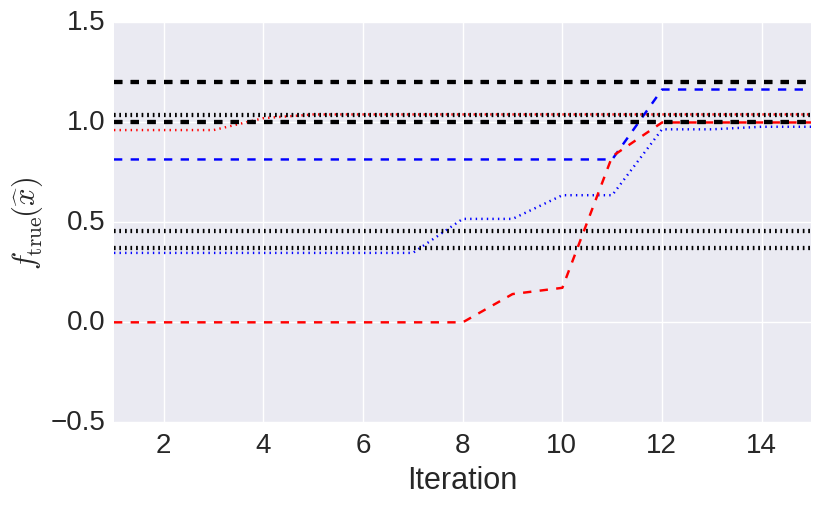
\includegraphics[width=0.6\textwidth]{figs/bayesopt/iteration_vs_error.png}&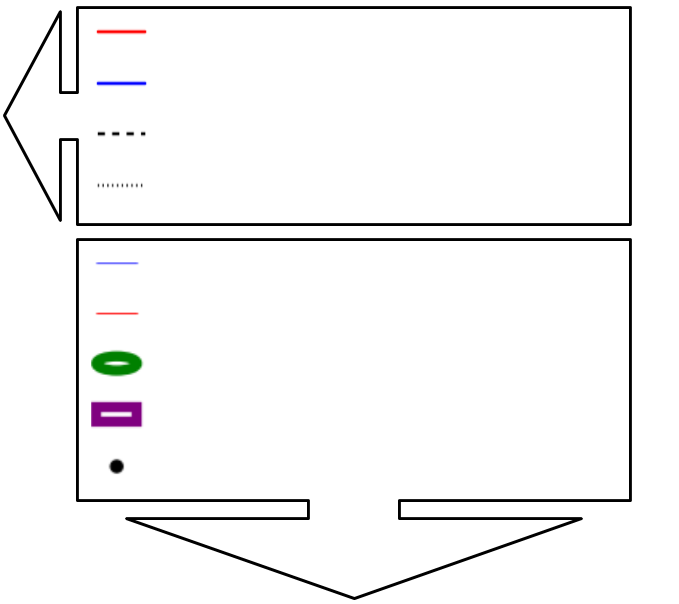
\includegraphics[width=0.4\textwidth]{figs/bayesopt/legend.png}
\put(-119,142){\scriptsize Drift Proposal}
\put(-119,130){\scriptsize Uniform Proposal}
\put(-119,117){\scriptsize Global Optimum}
\put(-119,105){\scriptsize Local Optima}
\put(-119,85){\scriptsize Ground Truth}
\put(-119,73){\scriptsize Posterior samples}
\put(-119,60){\scriptsize Next Probe}
\put(-119,48){\scriptsize Estimated Optimum}
\put(-119,36){\scriptsize Past Probes}
\end{tabular}
\begin{tabular}{llll}\hline 
\multicolumn{1}{|l|}{\raisebox{-0.5\height}{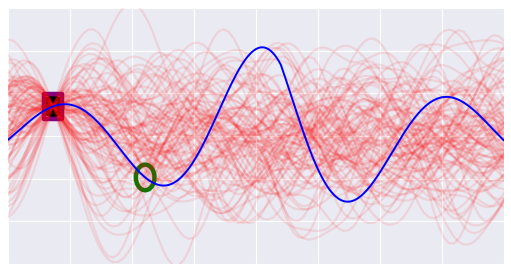
\includegraphics[width=0.3\textwidth]{figs/bayesopt/opt_sequence_uniform_trimodal_1.png}}}&
\multicolumn{1}{l|}{\raisebox{-0.5\height}{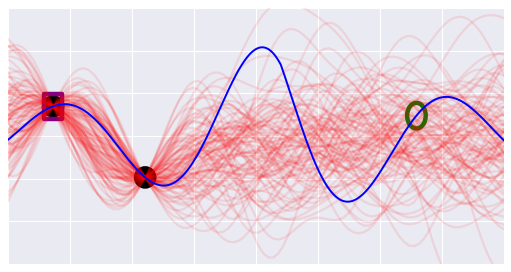
\includegraphics[width=0.3\textwidth]{figs/bayesopt/opt_sequence_uniform_trimodal_2.png}}}&
\multicolumn{1}{l|}{\raisebox{-0.5\height}{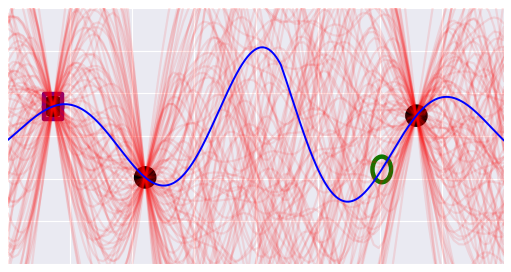
\includegraphics[width=0.3\textwidth]{figs/bayesopt/opt_sequence_uniform_trimodal_3.png}}} \\ \hline
\multicolumn{1}{|l|}{\raisebox{-0.5\height}{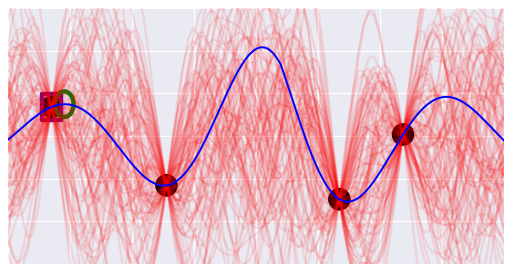
\includegraphics[width=0.3\textwidth]{figs/bayesopt/opt_sequence_uniform_trimodal_4.png}}}&
\multicolumn{1}{l|}{\raisebox{-0.5\height}{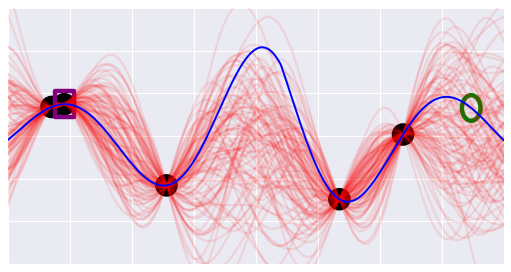
\includegraphics[width=0.3\textwidth]{figs/bayesopt/opt_sequence_uniform_trimodal_5.png}}}&
\multicolumn{1}{l|}{\raisebox{-0.5\height}{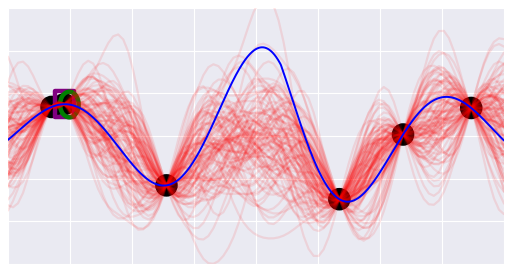
\includegraphics[width=0.3\textwidth]{figs/bayesopt/opt_sequence_uniform_trimodal_6.png}}} \\ \hline
\multicolumn{1}{|l|}{\raisebox{-0.5\height}{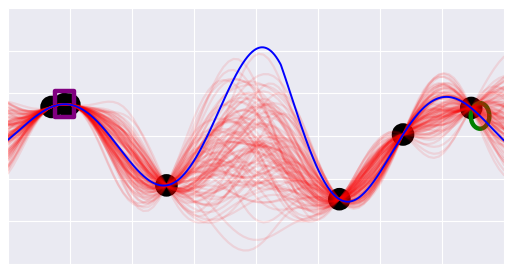
\includegraphics[width=0.3\textwidth]{figs/bayesopt/opt_sequence_uniform_trimodal_7.png}}}&
\multicolumn{1}{l|}{\raisebox{-0.5\height}{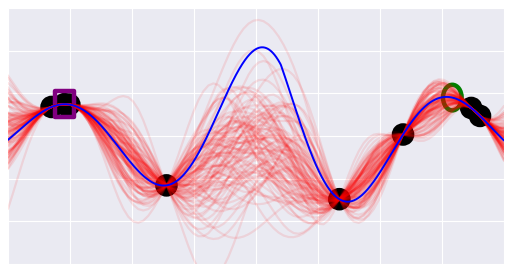
\includegraphics[width=0.3\textwidth]{figs/bayesopt/opt_sequence_uniform_trimodal_8.png}}}&
\multicolumn{1}{l|}{\raisebox{-0.5\height}{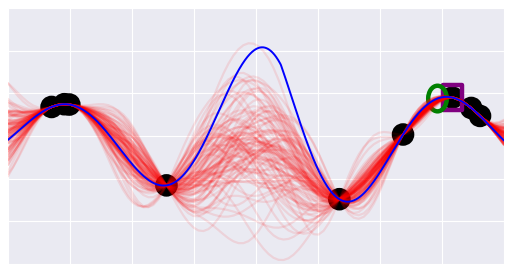
\includegraphics[width=0.3\textwidth]{figs/bayesopt/opt_sequence_uniform_trimodal_9.png}}} \\ \hline
\multicolumn{1}{|l|}{\raisebox{-0.5\height}{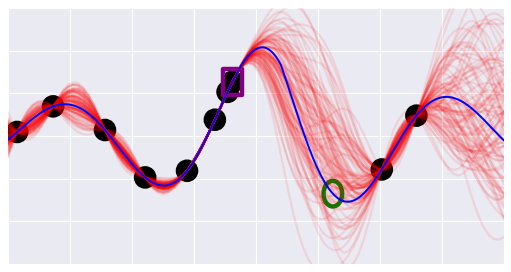
\includegraphics[width=0.3\textwidth]{figs/bayesopt/opt_sequence_uniform_trimodal_10.png}}}&
\multicolumn{1}{l|}{\raisebox{-0.5\height}{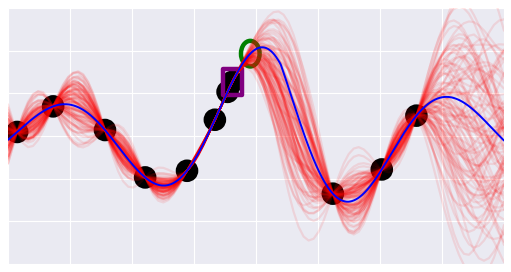
\includegraphics[width=0.3\textwidth]{figs/bayesopt/opt_sequence_uniform_trimodal_11.png}}}&
\multicolumn{1}{l|}{\raisebox{-0.5\height}{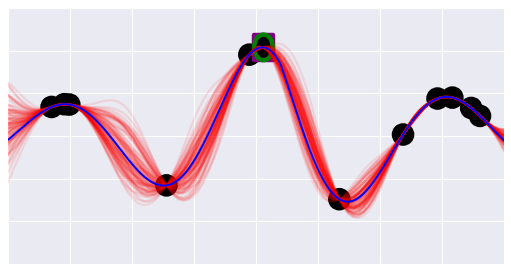
\includegraphics[width=0.3\textwidth]{figs/bayesopt/opt_sequence_uniform_trimodal_12.png}}} \\ \hline
\end{tabular}
\put(-387,130){\footnotesize$i = 2$}
\put(-255,130){\footnotesize$i = 3$}
\put(-123,130){\footnotesize$i = 4$}
\put(-387,62){\footnotesize$i = 5$}
\put(-255,62){\footnotesize$i = 6$}
\put(-123,62){\footnotesize$i = 7$}
\put(-387,-8){\footnotesize$i = 8$}
\put(-255,-8){\footnotesize$i = 9$}
\put(-123,-8){\footnotesize$i = 10$}
\put(-387,-78){\footnotesize$i = 11$}
\put(-255,-78){\footnotesize$i = 12$}
\put(-123,-78){\footnotesize$i = 13$}
\caption{Top: the estimated optimum over time. Blue and Red represent optimization with uniform and Gaussian drift proposals. Black lines indicate the local optima of the true functions. Bottom: a sequence of actions. Depicted are iterations 7-12 with uniform proposals.}\label{fig:bopt_results}
\end{figure}
In Fig. \ref{fig:bopt_results} we show results for our implementation of Bayesian Optimization 
with Thompson sampling. We compare two different proposal distributions, namely uniform proposals
and Gaussian drift proposals. We see that in this experiment, Gaussian drift is starting near 
the global optimum and drifts quickly towards it. (red curve, top panel of Fig. \ref{fig:bopt_results}).
Uniform proposals take longer to find the global optimum (blue curve, top panel of Fig. \ref{fig:bopt_results})
but we see that it can surpass the local optima of the curve\footnote{In fact, repeated experiments have
shown that when the Gaussian drift proposals starts near a local optimum, it gets stuck there. Uniform
proposals do not.}.
The bottom panel of Fig. \ref{fig:bopt_results} depicts a sequence of actions using uniform proposals.
The sequence illustrates the exploitation exploration trade-off that the implementation overcomes.
We start with complete uncertainty ($i=2$).
The Bayesian agent performs exploration until it gets a (wrong!) idea of where the optimum could be
(exploiting the local optima $i=5$ to $i=10$).
$i=11$ shows a change in tactic. The Bayesian agent, having exploited the local optima in previous
steps, is now reducing uncertainty in area it knows nothing about, eventually finding the global
optimum. 


